\chapter{User Flows}
\label{capitolo3}
In questa sezione vengono presentati gli User Flows correlati alla figura dell'Amministratore da noi scelta. La figura \ref{fig:userFlow} descrive lo User Flow relativo alla gestione ed ottenimento delle informazioni del parco, già introdotte nel capitolo introduttivo. In qualsiasi momento l'amministratore può gestire e visualizzare i sensori presenti nel parco e visualizzare informazioni inerenti la flora e la fauna del suddetto.

Nella figura \ref{fig:userFlow} vengono anche presentate le relazioni tra le azioni effettuate da parte dell'amministratore e le features descritte nel capitolo precedente. In aggiunta viene posta una legenda per facilitare la comprensione del diagramma sottostante.

%\newpage

\begin{figure}[ht]
    \centering
    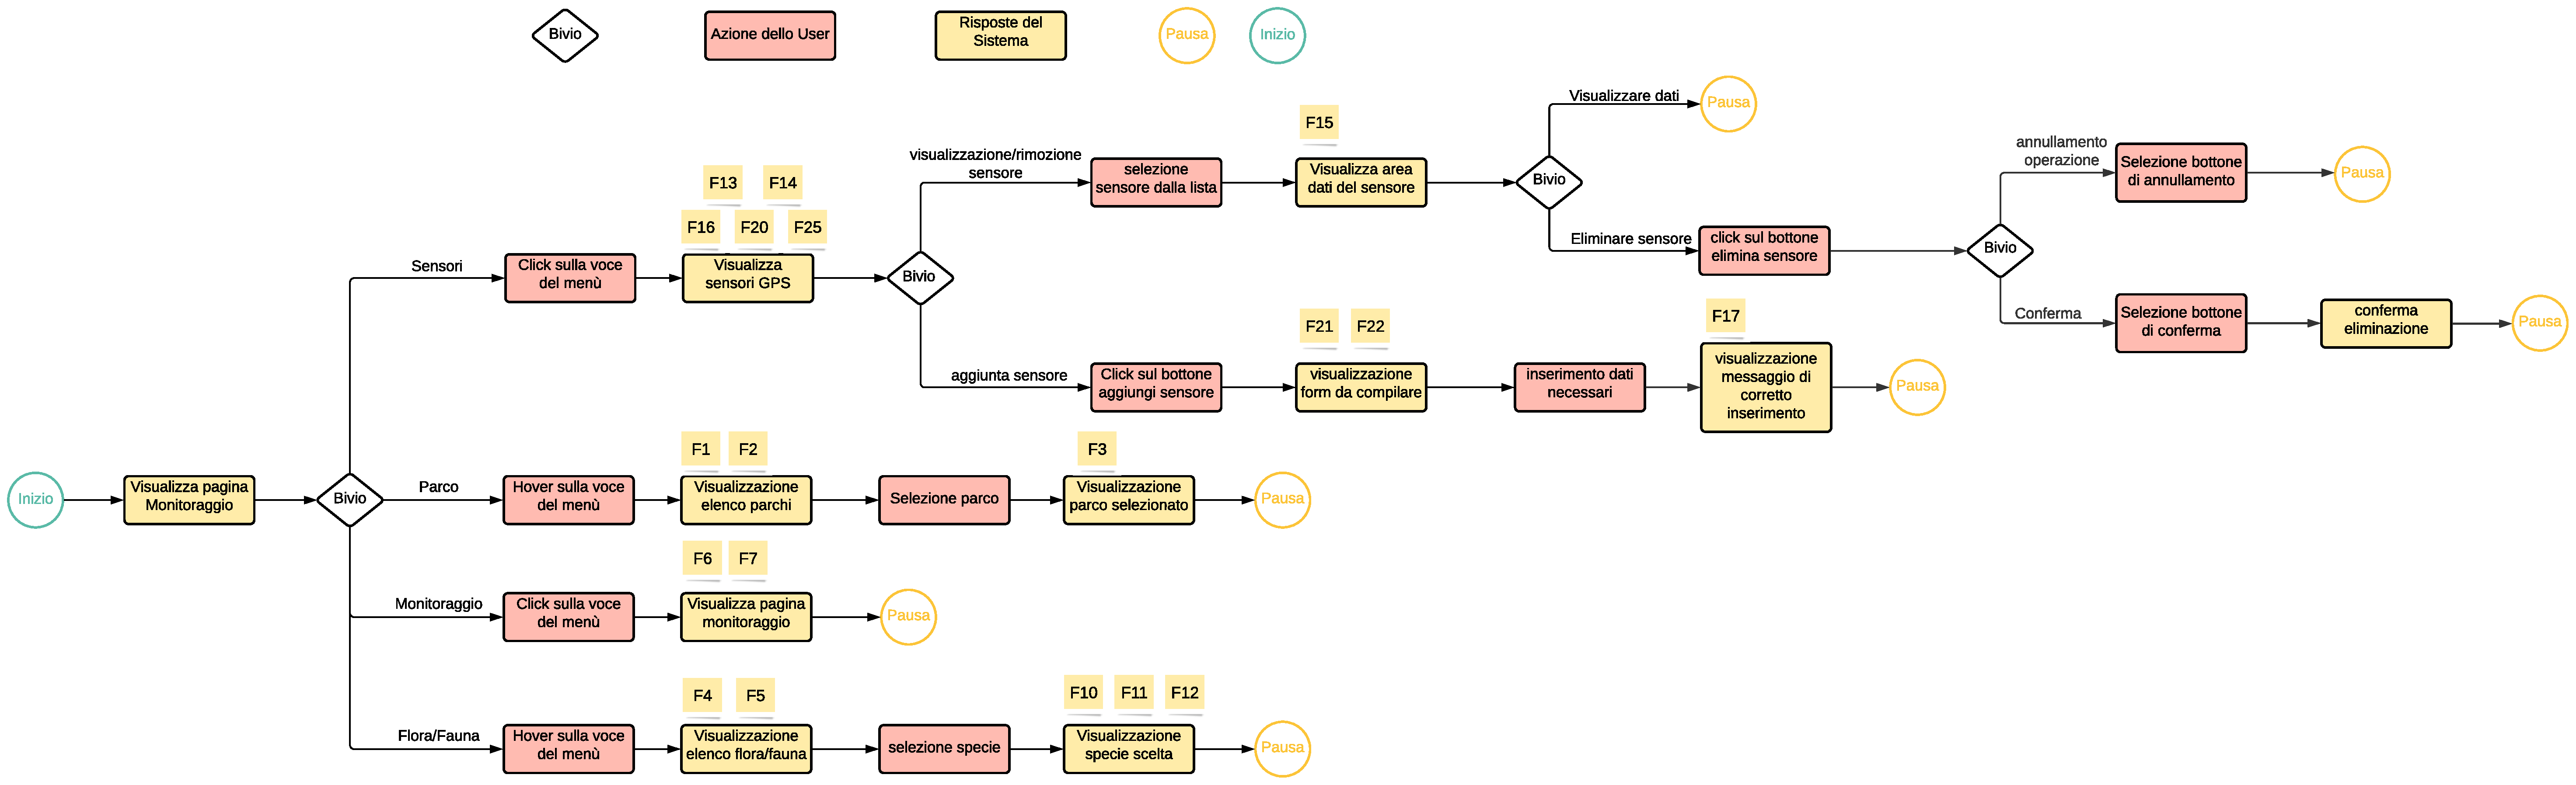
\includegraphics[scale=0.25,angle=90,origin=c]{Img/userFlow.eps}
    \caption{User flow}
    \label{fig:userFlow}
\end{figure}
